
%----------------------------------------------------------------
%
%  File    :  komponenten.tex
%
%  Authors :  ???
% 
%  Created :  7 Sept 2019
% 
%  Changed :  7 Sept 2019
% 
%---------------------------------------------------------------


\section{Komponenten}
\label{sec:Komponenten}

\subsection{State of the Art Marktanalyse}
\label{subsec:Marktanalyse}

Um die ansässigen Inselbewohner zufriedenzustellen, sollten insbesondere Peak Data Raten, die Zellkapazitäten, der Zellradius, die Radio Access Modi, die Antennen Schemata, sowie das Mobility Speed Handover konkreter in Erwägung gezogen werden\cite{Dat14}.
Bei der Recherche zur Thematik haben sich folgende Kriterien als Unterscheidungsmerkmale herauskristallisiert, welche eine Entscheidungsfindung beeinflussen. Ob nun anhand dieser letztlich eine Entscheidung getroffen wird, ob nun ein Mobilfunknetz selbst errichtet (Make) oder die notwendigen Komponenten (Buy) hinzugekauft werden sollen, wird im Kapitel Make or Buy näher beleuchtet. Neben dem Spektrum, dem Durchsatz (Throughput), der Latenz (Latency), der Redundanz (Redundancy), der Interoperabilität beziehungsweise der Kompatibilität, ist auch die Möglichkeit der Skalierbarkeit, um etwaige Nachbarinseln mitzuversorgen, von signifikanter Bedeutung. Denn diese haben ihrerseits kooperativ ihre Hilfe zur Analyse der Problematik in Form der Nutzung eines Internet Cafes angeboten, um erste Recherchearbeit bezüglich des Aufbaus eines LTE Mobilfunknetzes zu liefern. Zusätzlich  als weitere nicht zu vernachlässigende Elemente stellen auch Kriterien wie das des Monitorings respektive des Control Managements, ebenso wie dem möglichen Coverage, als auch die Kapazität Faktoren dar, welche die finalen Entscheidungsprozesse maßgeblich beeinflussen. Zudem sollte abzuwägen sein, ob ein "Easy to use Enterprise Dashboard" vorhanden ist. Des Weiteren wird die Art der Lizenz von Open Source Projekten, unter dem Aspekt der anschließenden Vermarktung, geprüft. Auch zu beachten ist, ob nach internationalem Recht bzw. in welchen gesetzlichen Rahmenbedingungen die verantwortlichen Projektleiter zu agieren haben.

%	\subsection{HSS, EPC, PCRF}
%	\label{subsec:Antennen HSS, EPC, PCRF}
%		\subsection{Preise der Komponenten}
%	\label{subsec:Preise der Komponenten}
	\subsection{Antennen Konfigurationen}
	\label{subsec:Antennen Konfigurationen}
Bevor man die Komponenten, welche von unterschiedlichen Marktteilnehmern angeboten werden vergleicht, ist es durchaus sinnvoll ein Bild über die Empfangsbedingungen in dem Inselstaat machen. Abhängig von physikalischen Einflussfaktoren in Form von Waldgebieten, Gebäudekomplexen oder topologischen Strukturen wie Gebirge sie darstellen, können ebensolche signifikant die Signalübertragung bestimmen. Denn schließlich sind Absorption, Beugung oder auch Reflexion mit die Hauptgründe für Störungen bei der Ausbreitung elektromagnetischer Wellen. Um nun einen optimalen Empfang zu gewähren kann eine Kombination aus Antennentypen angedacht werden, da jede einzelne Bauart ihre Vor- und Nachteile aufweist. So ist zu unterscheiden zwischen Mono- und Breitband Antennen. Mono-Antennen sind hierbei der Klasse der Richtantennen und Breitbandantennen der Klasse der Rundstrahler zuzuordnen. \cite{Sch19}
\begin{figure*}[ht]
	\centering
	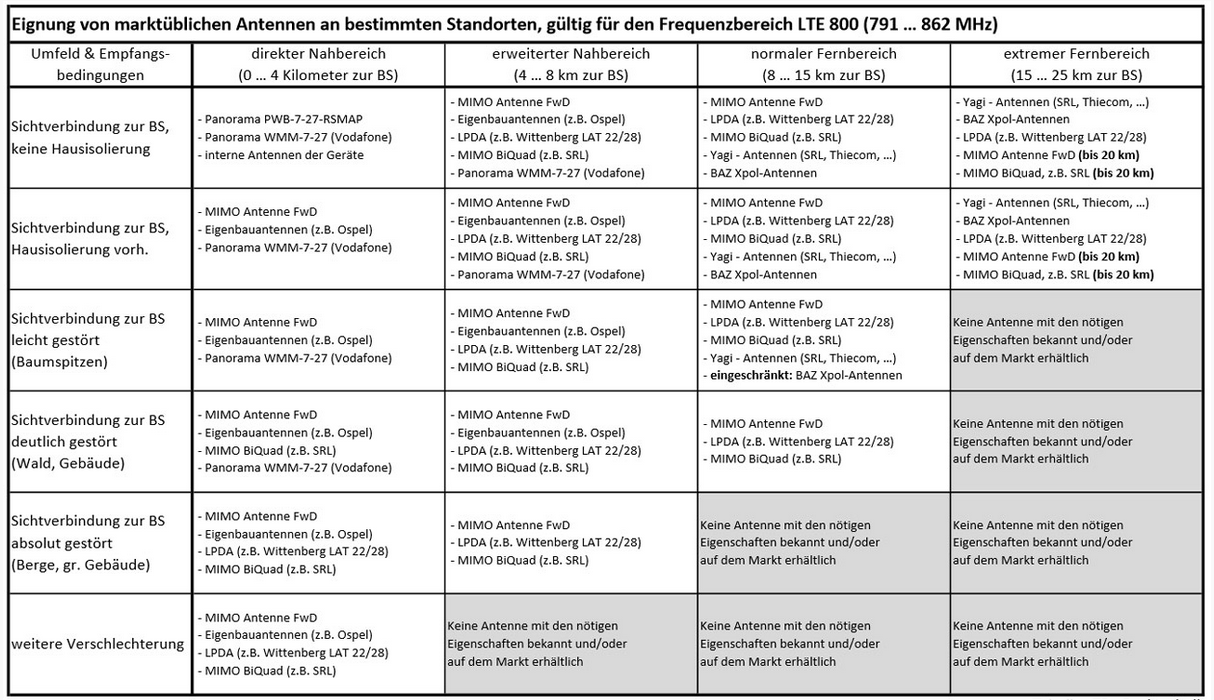
\includegraphics[width=1\linewidth]{images/tabellemcnantennen}
	\caption{Antennenüberblick  \protect\cite{Sch19}}
	\label{fig:tabellemcnantennen}
\end{figure*}
%\begin{figure*}[ht]
%	\centering
%	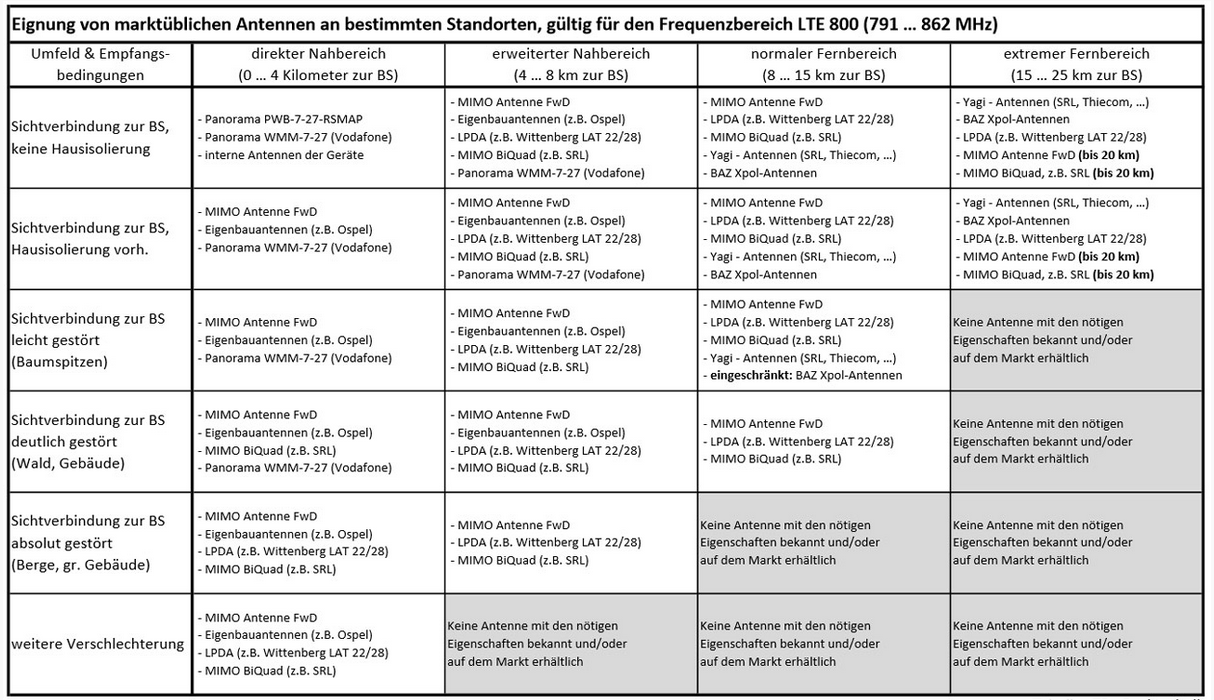
\includegraphics[width=1\linewidth]{images/tabellemcnantennen}
%	\caption{Antennenüberblick  \protect\cite{Sch19}}
%	\label{fig:tabellemcnantennen}
%\end{figure*}


%\newpage
 %\flushbottom 
%\nextpage
\raggedbottom 
